\documentclass[spanish, c]{beamer}

\usepackage[utf8]{inputenc}
% \usepackage[spanish, mexico]{babel}
\usepackage{amsmath}
\usepackage{mathtools}
\usepackage{hyperref}
\usepackage{xcolor}
\usepackage{color}
\usepackage{ragged2e}
\usepackage{mathrsfs}
% \usepackage{csquotes}
% \usepackage{listings}
\usepackage[scaled]{beramono}
\usepackage[T1]{fontenc}
\usepackage{graphicx}
\usepackage{booktabs}
\usepackage{physics}
\usepackage{minted}
\usepackage{tcolorbox}
\usepackage{tikz}
\usepackage{relsize}
\usepackage{algorithm}
\usepackage{algpseudocode}
\usepackage[shortlabels]{enumitem}
\usepackage{pifont}

\newcommand{\cmark}{\ding{51}}%
\newcommand{\xmark}{\ding{55}}%

\setlist[itemize]{label=\textbullet}  % global enumitem for default itemize

\tcbuselibrary{minted, skins}

\usetikzlibrary{arrows, automata, positioning, fit, shapes.geometric, backgrounds}
  
  \tikzset{
    stylename/.style={
      ->, %arrow type
      >=stealth', %arrow head type (bold)
      shorten >=1pt, 
      auto,
      %semithick,
      initial text=$ $, %no start text
    }
  }

\renewcommand{\indent}{\hspace*{2em}}

\newcommand\CC{C\nolinebreak[4]\hspace{-.05em}\raisebox{.4ex}{\relsize{-3}{\textbf{++}}}~}
\newcommand{\bigO}{\mathcal{O}}

\renewcommand{\Comment}[2][.55\linewidth]{%
  \leavevmode\hfill\makebox[#1][l]{\fontfamily{cmss}\selectfont\color{red}\footnotesize$\longrightarrow$\quad#2}}
% \usepackage{tikz}

% \usetikzlibrary{fit, shapes, arrows}

% \usepackage{courier}
% \usepackage{subfigure}
% \usepackage{enumerate}
% \usepackage{algorithmic}
% \usepackage{algorithm}

% \usepackage{listings}
% \usepackage{lstlinebgrd}

\usetheme{Boadilla}
\usefonttheme[onlymath]{serif}

\newcommand\blfootnote[1]{%
\begingroup
\renewcommand\thefootnote{}\footnote{#1}%
\addtocounter{footnote}{-1}%
\endgroup
}

\algrenewcommand\alglinenumber[1]{\footnotesize #1}

\makeatletter
% start with some helper code
% This is the vertical rule that is inserted
\newcommand*{\algrule}[1][\algorithmicindent]{%
  \makebox[#1][l]{%
    \hspace*{.2em}% <------------- This is where the rule starts from
    \vrule height .75\baselineskip depth .25\baselineskip
  }
}

\newcount\ALG@printindent@tempcnta
\def\ALG@printindent{%
    \ifnum \theALG@nested>0% is there anything to print
    \ifx\ALG@text\ALG@x@notext% is this an end group without any text?
    % do nothing
    \else
    \unskip
    % draw a rule for each indent level
    \ALG@printindent@tempcnta=1
    \loop
    \algrule[\csname ALG@ind@\the\ALG@printindent@tempcnta\endcsname]%
    \advance \ALG@printindent@tempcnta 1
    \ifnum \ALG@printindent@tempcnta<\numexpr\theALG@nested+1\relax
    \repeat
    \fi
    \fi
}
% the following line injects our new indent handling code in place of the default spacing
\patchcmd{\ALG@doentity}{\noindent\hskip\ALG@tlm}{\ALG@printindent}{}{\errmessage{failed to patch}}
\patchcmd{\ALG@doentity}{\item[]\nointerlineskip}{}{}{} % no spurious vertical space
% end vertical rule patch for algorithmicx
\makeatother
%

% Sets the templates
\definecolor{navyblue}{RGB}{0, 0, 128}
\definecolor{crimson}{RGB}{128, 16, 0}

\setbeamertemplate{navigation symbols}{}
\setbeamertemplate{headline}{}
\setbeamertemplate{title page}[default][colsep=-4bp,rounded=true]
\setbeamertemplate{footline}[frame number]
\setbeamertemplate{bibliography item}[text]
\setbeamertemplate{theorems}[numbered]

\setbeamercolor{title}{fg=navyblue, bg=white}
\setbeamercolor{frametitle}{fg=navyblue, bg=white}
\setbeamercolor{structure}{fg=navyblue}
\setbeamercolor{button}{fg=white,bg=navyblue}

\setbeamercovered{transparent}

\tcbset{cppexample/.style={%
    colback=green!5,
    colframe=green!30!black,
    listing only,
    fonttitle=\bfseries,
    listing engine=minted,
    minted language=c++,
    minted options={fontsize=\scriptsize, breaklines, linenos, autogobble, numbersep=2mm},
    enhanced,
    overlay={\begin{tcbclipinterior}\fill[red!25!green!25!white] (frame.south west)rectangle ([xshift=4mm]frame.north west);\end{tcbclipinterior}}
}}

\tcbset{cppfullexample/.style={%
    % colback=green!5,
    % colframe=green!30!black,
    listing only,
    fonttitle=\bfseries,
    listing engine=minted,
    minted language=c++,
    minted options={fontsize=\scriptsize, breaklines, linenos, autogobble, numbersep=2mm},
    enhanced,
    overlay={\begin{tcbclipinterior}\fill[black!20!white] (frame.south west)rectangle ([xshift=4mm]frame.north west);\end{tcbclipinterior}}
}}

\tcbset{cppfullborderless/.style={%
    % colback=green!5,
    % colframe=green!30!black,
    listing only,
    listing engine=minted,
    minted language=c++,
    minted options={fontsize=\scriptsize, breaklines, linenos, autogobble, numbersep=2mm},
    enhanced,
    overlay={\begin{tcbclipinterior}\fill[black!20!white] (frame.south west)rectangle ([xshift=4mm]frame.north west);\end{tcbclipinterior}}
}}

\title{Complejidad y problemas \texorpdfstring{$\mathcal{NP}$}{NP}}
\subtitle{Programación de Estructuras de Datos y Algoritmos Fundamentales \\ (TC1031)}
\author{
    \texorpdfstring{
        \begin{center}
            M.C. Xavier Sánchez Díaz \\
            \href{mailto:sax@tec.mx}{\texttt{sax@tec.mx}}
        \end{center}
    }
    {M.C. Xavier Sánchez Díaz}
}

\institute[Tecnológico de Monterrey]{\includegraphics[scale=0.5]{../img/logo}}
\date{}

\begin{document}

\setlength{\rightskip}{0pt}

\begin{frame}[plain]
    \titlepage        
\end{frame}

\begin{frame}{Outline}
    \tableofcontents
\end{frame}

\section{Recapitulación}

\begin{frame}{Órdenes más comunes}{Recapitulación}
    \begin{itemize}
        \item $\bigO(1)$ que es constante
        \item $\bigO(\log n)$ que es logarítmico
        \item $\bigO(n)$ que es \textit{lineal}
        \item $\bigO(n \log n)$
        \item $\bigO(n^2)$ que es \textit{cuadrático}
        \item $\bigO(n^2 log n)$
        \item $\bigO(n^m)$ que es \textit{polinomial}
        \item $\bigO(m^n)$ que es \textit{exponencial}
        \item $\bigO(n!)$ que es \textit{factorial}
    \end{itemize}
\end{frame}

\section{Introducción}

\begin{frame}{El cómputo}{Introducción}
    Las \textbf{ciencias computacionales} se encargan de estudiar el \textit{cómo} resolver los problemas (no las computadoras).
    A esto se le conoce como \alert{cómputo} y se relaciona directamente con todo lo que tiene que ver con \textit{cómo} generar \alert{cálculos}. \pause

    \bigskip

    \begin{itemize}
        \item ¿Podemos calcularlo todo? \pause
        \item ¿Qué información necesitamos para poder calcular la respuesta a alguna pregunta?
    \end{itemize}

\end{frame}

\begin{frame}[allowframebreaks]{Breve historia}{Introducción}

    \begin{itemize}
        \itemsep3.5ex
        \item En 1928, David Hilbert y Wilhelm Ackermann (GER) se cuestionan si es posible contestar a la pregunta:\\
        \begin{center}
            \textit{Si te doy un enunciado lógico, ¿hay alguna manera consistente de asegurar si el enunciado es universalmente válido?}
        \end{center}
        $$MagicBox(\Phi) = \begin{cases}0 & \text{si $\Phi$ no es válida} \\ 1 & \text{si $\Phi$ es válida}\end{cases}$$
        \item En 1935, Alonzo Church (US) genera un concepto abstracto de cómputo usando funciones ($\lambda$-calculus) que demuestra que no existe manera de saberlo.
        \item En 1936, Alan Turing (UK) genera un concepto abstracto de cómputo usando máquinas de estados (\textit{Turing Machines}) que demuestra que no existe manera de saberlo. Unos meses después, Turing demuestra que su sistema es equivalente al de Church.
        \item El método de Turing es más fácil de entender y explicar, y se acepta como estándar.
    \end{itemize}

    \begin{center}
        \LARGE Ejemplo: Stanford's CS103 de Keith Schwarz
    \end{center}

\end{frame}

\begin{frame}{Determinismo vs No-determinismo}{Introducción}
    
    La palabra \textbf{determinismo} hace referencia a que la solución a un problema se puede obtener después de un número \textbf{determinado} de pasos que depende del \textbf{estado} en el que se encuentra el problema. Algunas operaciones deterministas son: \pause
    
    \bigskip

    \begin{itemize}
        \item Sumar dos números \pause
        \item Multiplicar dos matrices \pause
        \item Ordenar una lista \pause
        \item Encontrar el número más pequeño en un arreglo
    \end{itemize}
\end{frame}

\begin{frame}
    \frametitle{Problemas \texorpdfstring{$\mathcal{P}$}{P}}
    \framesubtitle{Clases de complejidad}

    Si en su lugar, nos limitamos tener una máquina \alert{determinista} (es decir que sólo puede estar en un estado), entonces sólo algunos de los problemas $\mathcal{NP}$ se pueden resolver en un tiempo \textit{decente} ($\bigO(n^m)$)
    \begin{center}
        \Large A lo mucho, en tiempo \alert{polinomial}.
    \end{center}

    \begin{itemize}
        \item Son problemas de \textbf{decisión}: ¿Puedes? \textit{Yes or no}. \pause
        \item Se verifican \textbf{fácilmente}: si ya tengo una solución para comparar, puedo ver si voy por buen camino o si el problema está bien hecho.
        \item Se resuelven \textbf{siempre} con el mismo número de pasos (en el peor de los casos)
    \end{itemize}
\end{frame}

\begin{frame}{Determinismo vs No-determinismo}{Introducción}

    El \textbf{no-determinismo} es lo contrario. Considera el siguiente \textit{autómata no determinista} donde $\varepsilon$ es la palabra vacía (o sea \texttt{''}):

    \bigskip

    \begin{center}
        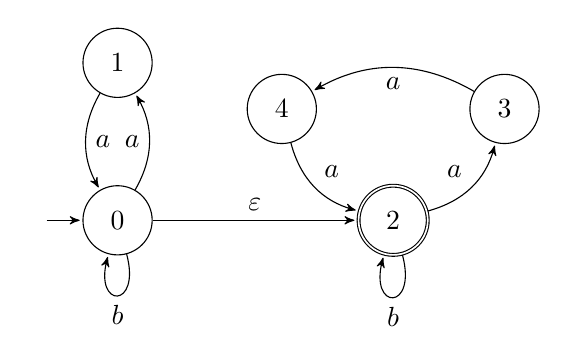
\begin{tikzpicture}[node distance=2cm, stylename]
          \node[initial, state] (0) {$0$};
          \node[state, above of=0] (1) {$1$};
          \node[state, accepting, right of=0, xshift=1.5cm] (2) {$2$};
          \node[state, above right of=2] (3) {$3$};
          \node[state, above left of=2] (4) {$4$};
    
          \path
          (0) edge [loop below] node {$b$} (0)
          (0) edge [bend right] node {$a$} (1)
          (0) edge node {$\varepsilon$} (2)
          (1) edge [bend right] node {$a$} (0)
          (2) edge [bend right] node {$a$} (3)
          (2) edge [loop below] node {$b$} (2)
          (3) edge [bend right] node {$a$} (4)
          (4) edge [bend right] node {$a$} (2);
        \end{tikzpicture}
      \end{center}
      
      La máquina está en \textbf{dos estados distintos a la vez} y las acciones siguientes dependen del estado en el que estás\dots que es en ambos\dots

\end{frame}

\begin{frame}
    \frametitle{Problemas \texorpdfstring{$\mathcal{NP}$}{NP}}
    \framesubtitle{Clases de complejidad}
    Si tuviéramos una máquina de ésas \alert{no deterministas} podríamos \textbf{decidir o verificar} si algunos problemas se pueden resolver en un tiempo \textit{decente} ($\bigO(n^m)$):
    \begin{center}
        \Large A lo mucho, en tiempo en \alert{polinomial}.
    \end{center} \pause
    \begin{itemize}
        \item Son también problemas de \textbf{decisión}
        \item Son también fácilmente \textbf{verificables}
    \end{itemize} \pause

    Se llaman $\mathcal{NP}$ por \textit{Non-deterministic Polynomial}, pueden ser resueltos y verificados por una máquina de Turing no determinista en un tiempo Polinomial ($\bigO(n^m$)).
\end{frame}

\begin{frame}[plain]
    \begin{center}
        \Huge
        \dots \\
        ¿Qué?
    \end{center}
\end{frame}

\begin{frame}
    \frametitle{Otra manera de ver a \texorpdfstring{$\mathcal{NP}$}{NP}}
    \framesubtitle{Clases de complejidad}

    Si ambos son de decisión y fácilmente verificables, ¿cómo sé si algún problema es $\mathcal{P}$ o es $\mathcal{NP}$?. \pause

    \begin{itemize}
        \item Los problemas en $\mathcal{P}$ los \textbf{resolvemos} con una máquina \alert{determinista} y los \textbf{verificamos} con \alert{la misma máquina} en tiempo \textbf{polinomial}. \pause
        \item Los problemas en $\mathcal{NP}$ los ```\textbf{resolvemos}''' con una máquina \alert{no determinista} pero los \textbf{verificamos} con una máquina \alert{determinista} en tiempo polinomial.
    \end{itemize}

\end{frame}

\begin{frame}[plain]

    \begin{center}
        Para cada uno de estos problemas pregúntate lo siguiente:
        
        \bigskip

        \textit{¿Es un problema de decisión?}

        \bigskip

        \textit{¿Puedo verificarlo rápidamente?}
        
        \bigskip

        \textit{¿Qué complejidad me toma?}

        \bigskip

        \textit{¿Si uso otro tipo de máquina reduzco el tiempo de solución?}
    \end{center}

\end{frame}

\begin{frame}{Ejemplos}{Clases de complejidad}
    
    \begin{description}[style=unboxed]
        \item [Armar un rompecabezas.]
         Si comparo cada una de las $n$ piezas contra todas las demás ($n-1$) entonces sé qué pieza va en cada lugar  $\rightarrow \bigO(n^2) \; {\color{green} \text{\cmark}}$ \pause
        \item [Sentar invitados en una mesa sin conflictos.]
        Por cada silla $n$ checo que no tenga conflicto con las $n-1$ sillas restantes. Luego, por la siguiente silla, checo con las $n-2$ restantes. Y así, o sea $n \times (n-1) \times (n-2) \dots = \bigO(n!) \; {\color{red} \text{\xmark}}$ \pause
        \item [Empacar la mayor cantidad de valores sin exceder la capacidad de una bolsa dados ciertos objetos de valor.] No es de decisión siquiera {\color{red} \xmark} \pause
        \item [Ordenar una lista de números.]
        El peor de los casos es que vengan en el orden contrario así que a lo mucho comparo todos contra todos los demás $\rightarrow \bigO(n^2) \; {\color{green} \text{\cmark}}$ \pause
        \item [Saber si un programa finalizará dada su instrucción inicial.] Es de decisión pero es imposible de resolver {\color{red} \xmark}
    \end{description}
\end{frame}

\begin{frame}{Ejemplos}{Clases de complejidad}
    
    \begin{description}[style=unboxed]
        \item [¿Puedes visitar todos los Starbucks de Monterrey de tal modo que la distancia que recorras sea la menor posible?.]
         Empiezo en uno, y me voy a alguno, y luego a otro y luego a otro\dots y anoto su distancia. Después empiezo en otro, y reviso las otras $n-1$ posibilidades, otras $n-2$ veces\dots $= \bigO(n!)$ {\color{red} \xmark}\pause
         \item [Asignar salones de clase a profesores.]
         Pruebo para uno de los $n$ profesores alguno de los $m$ salones disponibles y veo si no tiene problema a esa hora en ese salón. Luego reviso que no haya conflictos con los demás $n-1$ profesores en sus $m-1$ salones. Y asigno otro\dots $= \bigO(n!)$  {\color{red} \xmark} \pause
    \end{description}

    \begin{center}
        \Large
        ¿Notas algún patrón?
    \end{center}

\end{frame}

\begin{frame}{El no-determinismo de \texorpdfstring{$\mathcal{NP}$}{NP}}{Clases de Complejidad}

    Algunos de los que no se pueden resolver en tiempo polinomial podrían resolverse fácilmente si de manera \alert{no determinista} \textbf{generamos} una posible solución (\textit{good guess}) y la \textbf{verificamos} de manera \alert{determinista}.

    \bigskip

    Esos son los $\mathcal{NP}$.
    
    \bigskip

    ¿Puedes usar el mismo método para los $\mathcal{P}$? \pause
    
    Por supuesto, porque $\mathcal{P} \subseteq \mathcal{NP}$
\end{frame}

\section{Reducciones}

\begin{frame}{Resolver vs Verificar}{Reducciones}

    Ya vimos que \textbf{resolver} es más \textit{difícil} que \textbf{verificar}:

    \bigskip

    \begin{description}[style=unboxed]
        \itemsep3ex
        \item [Resolver un sudoku.]
        Tendrías que ir de cuadro en cuadro, probar con un número, y luego checar que dé la suma; y cambiar de uno por uno, para evitar conflictos con los $n-1$ restantes, que no tenga conflictos con los $n-2$ restantes\dots $= {\color{red} \bigO(n!)}$ \pause
        \item [Verificar la solución de un sudoku.]
        Recibo una solución propuesta y me voy de una por una en las $n$ casillas para revisar que todo cuadre. Si cuadra, perfecto. Si no, reporto que está mal. Esto toma ${\color{red} \bigO(n)}$ operaciones.
    \end{description}
\end{frame}

\begin{frame}{Una reducción absurda}{Reducción}

    Una \alert{reducción} es una transformación de un problema $easy$ a uno $harder$. Por ejemplo:
    
    \bigskip

    \begin{itemize}
        \item $easy = $ ``No puedo levantar este auto porque pesa demasiado'' \pause
        \item $harder = $ ``Me pregunto si podré levantar este barco de carga''
    \end{itemize} \pause

    \bigskip

    Por medio de una reducción, podemos convertir el problema $easy$ a un problema $harder$, por ejemplo pensando que metemos el auto \textit{dentro} del barco de carga. Si podemos levantar el barco de carga, entonces podemos levantar el auto. \pause

    \bigskip

    De este modo, resolver el problema $harder$ ayudó a resolver el problema $easy$.

\end{frame}

\begin{frame}{Reducción en tiempo polinomial}{Reducción}
    Haciendo una serie de \textit{transformaciones} a cualquiera de \textit{nuestros} problemas $\mathcal{NP}$ podemos hacer la siguiente \textit{máquina} (algoritmo): \pause

    \bigskip

    \begin{enumerate}[1.]
        \item Probemos todas las posibles soluciones para nuestro problema. \pause
        \item Si una de ellas termina, entonces detente. Si no, entra en un bucle infinito.
    \end{enumerate} \pause

    \bigskip

    Claramente, si el programa de 2 líneas se detiene significa que nuestro problema $\mathcal{NP}$ tenía una solución óptima.
\end{frame}

\begin{frame}{Reducción en tiempo polinomial}{Reducción}

    Esta reducción de nuestro problema $\mathcal{NP}$ a este otro problema de \textit{detener la máquina} nos dice entonces que \textbf{decidir si la máquina se detendrá} es \alert{más difícil} que resolver el problema $NP$ (o sea, es el barco de carga de nuestro auto). \pause

    \bigskip
    
    También podemos asegurar que resolver el problema $\mathcal{NP}$ (cargar nuestro auto) es \textit{al menos} \alert{tan difícil} como resolver el problema de \textbf{decidir si la máquina se detendrá}.
\end{frame}

\begin{frame}{\texorpdfstring{$\mathcal{NP}$}{NP}-hard}{Clases de complejidad}
    
    El problema de decidir si la máquina se va a detener o no dependiendo del programa (algoritmo) que recibe pertenece a la clase $\mathcal{NP}$-\textit{hard} o $\mathcal{NP}$-difícil. \pause

    \bigskip

    \begin{block}{$\mathcal{NP}$-\textit{hardness}}
        Un problema $X$ es $\mathcal{NP}$-\textit{hard} si todo problema $L \in \mathcal{NP}$ se puede reducir a $X$ en tiempo polinomial.
    \end{block}

    \bigskip
    
    Esto nos da una cadenita de complejidad interesante\dots
\end{frame}

\begin{frame}{Completez de $NP$}{Clases de complejidad}

    \begin{description}[style=unboxed]
        \item [Si un problema $L$ puede reducirse a otro que está en $P$, entonces $L \in \mathcal{P}$] que es la clase de los problemas eficientemente resolubles en tiempo polinomial.
        \item [Si un problema $L$ puede reducirse a otro que está en $\mathcal{NP}$, entonces $L \in \mathcal{NP}$] que es la clase de los problemas eficientemente verificables en tiempo polinomial.
        \item [Si un problema $L$ puede reducirse a otro que está en $\mathcal{NP}$-\textit{hard}, entonces $L \in \mathcal{NP}$-\textit{hard}] que es la clase de los problemas difíciles de resolver para \textbf{cualquier} \textit{computadora} (incluso aquellos que no puede resolver o son \textit{indecidibles}).
    \end{description}

    \bigskip

    \begin{block}{$\mathcal{NP}$-\textit{completeness}}
        Un problema $L$ que puede reducirse a un $\mathcal{NP}$, y que también puede reducirse a un $\mathcal{NP}$-\textit{hard} es un problema $\mathcal{NP}$-\textit{Complete} o $\mathcal{NP}$-\textit{Completo}
    \end{block}
\end{frame}

\begin{frame}{\texorpdfstring{$\mathcal{NP}$}{NP}-Complete}

    Los problemas $\mathcal{NP}$-\textit{Complete}, como pueden ser reducidos a $\mathcal{NP}$-\textit{hard}, también pueden servir para otras reducciones:

    \begin{itemize}
        \item Todos los problemas $\mathcal{NP}$-\textit{Complete} son \textbf{reducibles entre sí}---encontrar una manera eficiente de resolver óptimamente uno de ellos resuelve todos los demás.
        \item Todos los algoritmos para ```resolver''' los problemas $\mathcal{NP}$-\textit{Complete} corren en tiempo exponencial (o más).
        \item Todos los algoritmos para resolver los problemas $\mathcal{NP}$-\textit{Complete} no son factibles para una cantidad razonable de tamaño de problema $n$.
    \end{itemize}

\end{frame}

\begin{frame}{Volviendo a nuestros problemas propuestos}{Clases de complejidad}

    \begin{description}[style=unboxed]
        \item [Armar un rompecabezas]
         es un problema $\mathcal{P}$ porque es fácilmente resoluble fácilmente verificable \pause
        \item [Sentar invitados en una mesa sin conflictos]
        es un problema $\mathcal{NP}$ porque es fácilmente verificable, pero no es fácilmente resoluble. De hecho, es una instancia de la asignación de salones y es reducible al de saber si la máquina se detuvo por lo que es $\mathcal{NP}$-\textit{complete} \pause
        \item [Empacar la mayor cantidad de valores sin exceder la capacidad de una bolsa dados ciertos objetos de valor] no es de decisión así que no está en $\mathcal{NP}$. Sin embargo, la versión de decisión (puedo o no empacar esto\dots) es $\mathcal{NP}$-\textit{complete}, por lo que se considera $\mathcal{NP}$-\textit{hard} \pause
        \item [Ordenar una lista de números] es fácilmente resoluble y verificable\dots es $\mathcal{P}$ \pause
        \item [Saber si un programa finalizará dada su instrucción inicial] es $\mathcal{NP}$-\textit{hard} y es indecidible (o sea que no es posible resolverlo)
    \end{description}

\end{frame}

\begin{frame}{Volviendo a nuestros problemas propuestos}{Clases de complejidad}
    
    \begin{description}[style=unboxed]
        \itemsep3ex
        \item [Visitar todos los Starbucks de Monterrey de tal modo que la distancia que recorras sea la menor posible]
        es un problema $\mathcal{NP}$-\textit{complete} ya que es reducible a otros $\mathcal{NP}$-\textit{complete} \pause
        \item [Asignar salones de clase a profesores]
        es también $\mathcal{NP}$-\textit{complete} ya que se puede reducir a otro $\mathcal{NP}$-\textit{complete} como la asignación de asientos sin conflictos o la selección de objetos para empacado \pause
    \end{description}

\end{frame}

\begin{frame}{Más ejemplos de \texorpdfstring{$NP$-\textit{complete}}{NP-complete}}{Clases de complejidad}
    
    Hay muchísimos más $\mathcal{NP}$-\textit{complete} en la vida diaria:

    \begin{itemize}
        \itemsep 3.5ex
        \item ¿Si compro 5 torres de comunicaciones me garantiza que tengo cobertura suficiente para toda la ciudad? \pause
        \item ¿Hay alguna secuencia de 100 genes que sea común entre individuos de un grupo de tiras de ADN? \pause
        \item Dada una lista de precios y un presupuesto, ¿puedo comprar más de 15 objetos con ello? \pause
        \item Dada la distribución demográfica de una ciudad, ¿puedo usar 330,000 metros de tuberías para brindar agua a toda la población?
    \end{itemize}

\end{frame}

\begin{frame}{\texorpdfstring{$\mathcal{P} = \mathcal{NP}$}{P = NP}}{Clases de complejidad}

    \begin{center}
        \large
        ¿Existe alguna manera eficiente de resolver algún problema fácilmente verificable?\\
        Es decir, alguno de los $\mathcal{NP}$-\textit{complete} puede ser resuelto en tiempo polinomial?
    \end{center}

    \bigskip

    \begin{itemize}
        \item Es un problema abierto hasta el momento---no existe respuesta alguna a esta pregunta
        \item Se cree que no es el caso (y que por tanto $\mathcal{P} \neq \mathcal{NP}$) pero nadie ha logrado demostrarlo
        \item El Clay Institute of Mathematics ofrece \$ 1,000,000.00 USD a quien pueda resolverlo, y es uno de los problemas del milenio (quizá el más importante por todo lo que implica)
        \item Ha habido más de 100 intentos de pruebas para demostrar que $\mathcal{P}$ y $\mathcal{NP}$ son clases distintas; todas han fallado en ser correctas
    \end{itemize}

\end{frame}

% \section*{Referencias}

% \begin{frame}[t]{Referencias}
    % \nocite{bibID01}
    % \nocite{bibID02}

    % \bibliographystyle{IEEE}
    % \bibliography{biblio}
% \end{frame}

\end{document}